\documentclass{article}
\usepackage{tikz}
\usepackage{calculator}
\usepackage[outline]{contour}
\usepackage{amsmath}
\usepackage{amssymb}
\contourlength{2pt}
\usetikzlibrary {arrows.meta, shapes.geometric, automata, positioning, math, calc}

\tikzset{
	beginning/.pic={
		\draw [pic actions] (0,0) -- (1,1) -- (3,1) -- (3,0) -- (0,0);
	}
}

\tikzset{
	end/.pic={
		\draw [pic actions] (0,0) -- (1,0) -- (0,1) -- (0,0);
	}
}

\begin{document}

\newcommand\f{0.15}

\begin{equation}
	x_t = h(\rho x_{t-T_M}) + h((1 - \rho) x_{t-T_m})
\end{equation}

\begin{equation}
	f(t) = h(\rho f(t-T_M) + (1 - \rho) f(t-T_m))
\end{equation}

\begin{math}
	T_M = 2, T_m = 1
\end{math}

\begin{equation}
	f(3) = h(\rho f(1) + (1 - \rho) f(2))
\end{equation}

\begin{equation}
	f(4) = h(\rho f(2) + (1 - \rho) h(\rho f(1) + (1 - \rho) f(2)))
\end{equation}

\begin{equation}
	f(t) = \sum_{k=0}^{\lfloor \frac{t}{T_m} \rfloor}\left(f(t - kT_m + \lfloor \frac{t}{T_M} \rfloor T_M)\frac{(\lfloor \frac{t}{T_M} \rfloor + k)!}{ \lfloor \frac{t}{T_M} \rfloor ! k!}(1 - \rho)^{k} \rho^{\lfloor \frac{t}{T_M} \rfloor}\right)
\end{equation}

\begin{equation}
	f(t) = \sum_{k=0}^{n}\left(f(t - kT_m - nT_M)\binom{n+k}{k} (1 - \rho)^{k} \rho^n\right)
\end{equation}

\vspace{2cm}

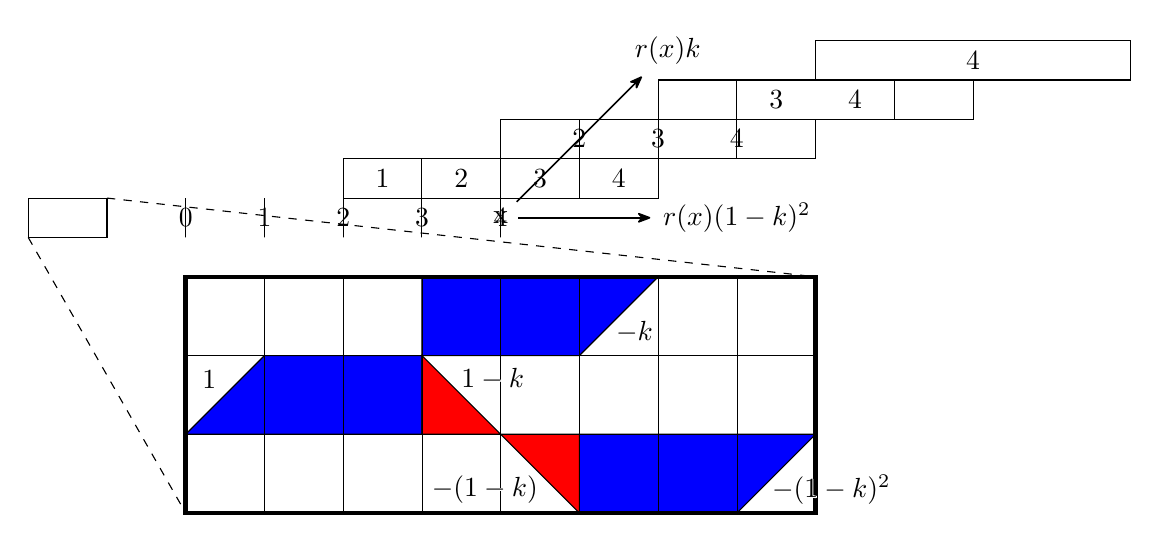
\begin{tikzpicture}
	\foreach \x  in {0, ..., 4} {
			\foreach \y in {0,...,\x}{

					\newcommand\varx{\x-\y*\f}
					\ADD{\x}{0}{\xplus};
					\draw (\varx-2, \y/2+3.5) rectangle node {$\xplus$} (\varx-1, \y/2+4);
				};
		};

% m=3 m-(k-1)
% n -					(m-0)	T_N,	k=0
% n - kT_F	- (m-1)	T_N,	k=1
% n - kT_F	- (m-2)	T_N,	k=2
% n - kT_F	- (m-3)	T_N,	k=3
% n - kT_F,								k=4

	\coordinate(spotlight1) at (-2, 3.5);
	\coordinate(spotlight2) at (-1, 4);
	\coordinate(spotlight3) at (0,0);
	\coordinate(spotlight4) at (8,3);

	\begin{scope}[->,>={Stealth[round]}, node distance=3cm, shorten >=1pt, auto, on grid, semithick]
		\node (a) at (4,3.75) {x};
		\node [above right=of a] (short) {$r(x)k$};
		\node [right=of a] (long) {$r(x)(1-k)^2$};

		\path (a) edge (short);
		\path (a) edge (long);
	\end{scope}

	\draw (spotlight1) rectangle node {} (spotlight2);

	\path [dashed] (spotlight1) edge (spotlight3);
	\path [dashed] (spotlight2) edge (spotlight4);

	\pic at (0,1) [fill=blue] {beginning};
	\pic at (3,1) [fill=red] {end};
	\pic at (8,1) [fill=blue, rotate=180] {beginning};
	\pic at (5,1) [fill=red, rotate=180] {end};
	\pic at (6,3) [fill=blue, rotate=180] {beginning};

	\draw [help lines, color=black] (spotlight3) grid (spotlight4);
	\draw[ultra thick] (spotlight3) rectangle (spotlight4);

	\node at (0.3, 1.7) {\contour{white}{$1$}};
	\node at (5.7, 2.3) {\contour{white}{$-k$}};
	\node at (3.9, 1.7) {\contour{white}{$1-k$}};
	\node at (3.8, 0.3) {\contour{white}{$-(1-k)$}};
	\node at (8.2, 0.3) {\contour{white}{$-(1-k)^2$}};

\end{tikzpicture}

\vspace{2cm}

\begin{tikzpicture}


\end{tikzpicture}

\vspace{2cm}

\newcommand\finger{0.3}

\begin{tikzpicture}
	\foreach \n  in {0, ..., 6} {
			\foreach \f in {0,...,\n}{
					\tikzmath{
						int \boxtext;
						\boxtext = \n + 1 - \finger * \f;
						\x = \n - \f * \finger;
					};

					\draw (\x, \f / 2) rectangle node {$\boxtext$} (\x + 1, \f / 2 + 0.5);
				};
		};
\end{tikzpicture}

% \tikz \draw (0,0) node {$r(x)(1-k)^2$} -- (1,0);
% \tikz \draw (0,0) node {$r(x)k$} -- (1,1);

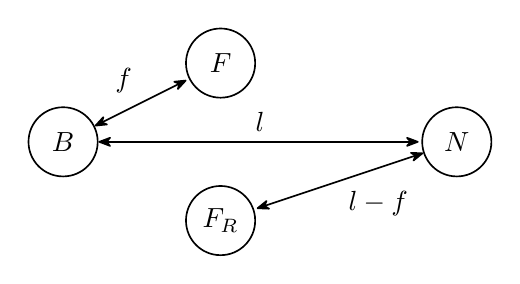
\begin{tikzpicture}[<->,>={Stealth[round]},shorten >=1pt,auto,node distance=2.8cm,on grid,semithick]

	\node[state] (B) at (0,0)		{$B$};
	\node[state] (F) at (2,1)		{$F$};
	\node[state] (R) at (2,-1)	{$F_R$};
	\node[state] (N) at (5,0)		{$N$};

	\path (B) edge node {$l$}		(N);
	\path (B) edge node {$f$}		(F);
	\path (N) edge node {$l-f$}	(R);
\end{tikzpicture}

\begin{math}
	P_r(n) = \frac{n(n+1)(n+2)(n+3)\cdots(n+r-1)}{r!}
\end{math}

\begin{math}
	n(n+1)(n+2)(n+3)\cdots(n+r-1) = \frac{(n+r-1)!}{(n-1)!}
\end{math}

\begin{math}
	r(r+1)(r+2)\cdots(n+r-1)r! = (n+r-1)!
\end{math}

\vspace{2cm}

\begin{equation}
	S_{out}(t) = \sum_{f=0}^{\lfloor \frac{T_f}{t} \rfloor}\left(S_{in}(t + f(T_n - T_f))\frac{(\lfloor \frac{T_n}{t} \rfloor + f)!}{ \lfloor \frac{T_n}{t} \rfloor ! f!} (1 - \rho)^{f} \rho^{\lfloor \frac{T_n}{t} \rfloor}\right)
\end{equation}

$ 0 \leq \rho \leq 1 $

\vspace{7mm}

\begin{equation}
	f_{out}(t) = \sum_{k=0}^{\lfloor \frac{t}{T_m} \rfloor}\left(f_{in}(t + k(T_M - T_m))\binom{\lfloor \frac{t}{T_M} \rfloor + k}{k}(1 - \rho)^{k} \rho^{\lfloor \frac{t}{T_M} \rfloor}\right)
\end{equation}

\begin{equation}
	f_{out}(t) = \sum_{k=0}^{\lfloor \frac{t}{T_m} \rfloor}\left(f_{in}(t - kT_m + \lfloor \frac{t}{T_M} \rfloor T_M)\binom{\lfloor \frac{t}{T_M} \rfloor + k}{k}(1 - \rho)^{k} \rho^{\lfloor \frac{t}{T_M} \rfloor}\right)
\end{equation}

\vspace{2cm}

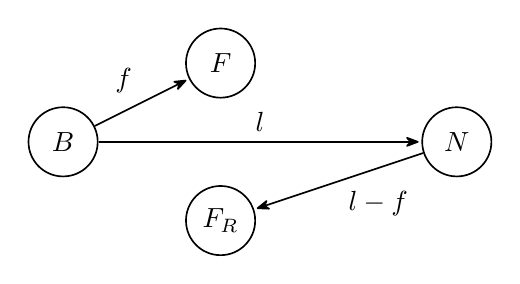
\begin{tikzpicture}[->,>={Stealth[round]}, shorten >=1pt, auto, node distance=2.8cm, on grid, semithick]

	\node[state] (B) at (0,0)		{$B$};
	\node[state] (F) at (2,1)		{$F$};
	\node[state] (R) at (2,-1)	{$F_R$};
	\node[state] (N) at (5,0)		{$N$};

	\path (B) edge node {$l$}		(N);
	\path (B) edge node {$f$}		(F);
	\path (N) edge node {$l-f$}	(R);
\end{tikzpicture}

\tikzset{%
	block/.style = { draw,
			thick,
			rectangle,
			minimum height = 2em,
			fill=white,
			align=center
		},
	wide block/.style = {
			block,
			text width=2.5cm,
			minimum width = 8em,
		},
	adder/.style={draw,circle},
	mul/.style={isosceles triangle,
			draw,
			fill=white,
			minimum size = 1em
		},
	branch/.style={fill,circle,minimum size=2pt,inner sep=-1pt},
}

\begin{tikzpicture}[auto, thick, node distance=2cm, >=Triangle]
	\node[block] (delayF1) {Delay $\frac{T_f}{2}$};
	\node[wide block, right = 40mm of delayF1] (delayN1) {Delay $\frac{T_n - T_f}{2}$};

	\node[block, below=20mm of delayF1] (delayF2) {Delay $\frac{T_f}{2}$};
	\node[wide block, below=20mm of delayN1] (delayN2) {Delay $\frac{T_n - T_f}{2}$};

	\node[branch](split) at ($(delayF1)!1/3!(delayN1)$) {};
	\node[adder](add) at ($(delayF2)!1/3!(delayN2)$) {+};
	\draw[-stealth](split) -- (add);

	\draw[-stealth](delayF1) -- (delayN1);
	% \node[above = 5mm of mm] {$1-\rho$};

	\draw[-stealth](delayN1.east) -- ++(1,0) |- (delayN2);
	\draw[-stealth](add)--(delayF2);
	\draw[-stealth] (delayN2) -- (add);

	\node[mul](l) at ($(split.east)!1/2!(delayN1.west)$) {};
	\node[above=.5em of l] {$\rho$};

	\node[mul, rotate = -90](finger) at ($(split.south)!1/2!(add.north)$) {};
	\node[right=.5em of finger] {$1-\rho$};

	\node[mul, rotate = -90, yshift=28](nut) at ($(delayN1.east)!1/2!(delayN2.east)$) {};
	\node[right=.5em of nut] {$-1$};

	\node[block, left=8mm of delayF2] (filter) at ($(delayF1)!1/2!(delayF2)$) {Round-trip \\ filter};

	\node[branch](outsplit) at (filter |- delayF2) {};

	\draw[-stealth](delayF2.west) -- node[below left]{output} ++ (-2,0);
	\draw[-stealth](outsplit) -- (filter.south);
	\draw[-stealth](filter.north) |- (delayF1.west);
\end{tikzpicture}

A plucked modelled as two delay lines 

Let the initial signal $S_{in}(t)$. There are two mechanisms of energy losses occurring on the input signal while it goes through the string. The scattering losses and the propagation losses. Since there are two types of roundtrips, the F-roundtrip (finger roundtrip) and the N-roundtrip (nut roundtrip), we assume that their corresponding loss coefficients are $a$ and $b$.

Consider next a case where  n roundtrips of types $F$ and $N$ respectively. The total number of such $m$ roundtrips is determined by considering the combinatorial problem of choosing $f$ scatterings of $F$ type out the off total $m = f + n$ scatterings. The answer is $\binom{m}{f}$. Equivalently we could ask the combinatorial problem of choosing n roundtrips of $N$ type out of the total $m = f + n$ roundtrips.


\end{document}

